\chapter{Dynamique relativiste}\label{ch:b3:relativistic-dynamics}

En 1964, William Bertozzi filma des électrons lancés dans un
accélérateur linéaire~: chaque paquet recevait une énergie mesurée, et
sa vitesse était chronométrée sur \qty{8.4}{m} de vol. Newton prédisait
que des électrons de \qty{15}{MeV} devaient voler à huit fois la
vitesse de la lumière~; le chronomètre annonça $0.9999c$ et refusa
d'aller plus loin, si fort que l'on poussât les électrons. La
cinématique nous a dit au chapitre précédent que $c$ est une limite~;
la dynamique doit maintenant expliquer ce qu'il advient de la poussée
--- où passe le travail quand la vitesse ne croît plus. La réponse
réorganise la mécanique autour d'une nouvelle quantité de mouvement et
d'une nouvelle énergie, réunies dans l'équation la plus célèbre de la
physique~: l'énergie stockée est de la masse, la masse est de l'énergie
en résidence, $E = mc^2$. Ce chapitre construit cette dynamique, puis
la met au travail là où elle vit chaque jour --- désintégrations
radioactives, collisions de particules, et les accélérateurs qui
changent du mouvement en matière neuve.

\section{Quantité de mouvement et énergie, refondues}

\begin{remark}[Pourquoi $m\vect v$ devait céder]\label{rem:b3:relativistic-dynamics:why}
La quantité de mouvement classique $m\vect v$ se conserve dans tout
référentiel \emph{si} les vitesses se transforment à la manière de
Galilée. Elles ne le font pas
(\cref{prop:b3:relativistic-kinematics:addition})~: une collision qui
conserve $\sum m\vect v$ dans un référentiel ne la conserve pas dans un
autre, si bien que l'ancienne quantité de mouvement ne peut être une
loi de la nature --- tout au plus l'ombre, aux faibles vitesses, d'une
loi véritable. La réparation consiste à mesurer la vitesse avec
l'horloge \emph{propre} de la particule~: $\dd\vect r/\dd\tau =
\gamma\,\vect v$ se transforme proprement, et $m\,\dd\vect r/\dd\tau$
se trouve conservé dans tous les référentiels à la fois.
\end{remark}

\begin{definition}[Quantité de mouvement et énergie relativistes]\label{def:b3:relativistic-dynamics:momentum-energy}
\index{quantité de mouvement relativiste}\index{énergie relativiste}\index{énergie de masse}
Une particule de masse $m$ et de vitesse $\vect v$ ($\gamma = 1/\sqrt{1 -
v^2/c^2}$) porte la quantité de mouvement et l'énergie
\[
\vect p = \gamma m\vect v , \qquad
E = \gamma mc^2 .
\]
Au repos, $E_0 = mc^2$~: l'\emph{énergie de masse}. L'énergie cinétique
est ce que le mouvement ajoute, $E_k = E - mc^2 = (\gamma - 1)mc^2$, qui pour $v
\ll c$ se réduit au familier $\tfrac12 mv^2$ (développer $\gamma$).
Dans tout processus isolé, la $\vect p$ totale et l'$E$ totale ---
énergies de masse comprises --- sont conservées.
\end{definition}

\begin{theorem}[La relation énergie--impulsion]\label{thm:b3:relativistic-dynamics:relation}
\index{relation énergie--impulsion}
Pour toute particule,
\[
E^2 = (pc)^2 + (mc^2)^2 ,
\qquad
\vect v = \frac{\vect p\,c^2}{E} :
\]
la combinaison $E^2 - p^2c^2 = m^2c^4$ prend la même valeur dans tout
référentiel --- elle est à l'énergie et à la quantité de mouvement ce
que l'intervalle est au temps et à l'espace. Deux régimes~: à faible
vitesse, $E \approx mc^2 + p^2/2m$~; à haute énergie ($E \gg mc^2$),
$E \approx pc$ et $v \to c$~: pousser plus fort ajoute de l'énergie et
de la quantité de mouvement, presque pas de vitesse.
\end{theorem}

\begin{proof}
$E^2 - p^2c^2 = \gamma^2m^2c^4(1 - v^2/c^2) = m^2c^4$~; et $pc^2/E =
\gamma mvc^2/\gamma mc^2 = v$. L'invariance de référentiel suit de ce
que $m$ et $c$ n'en dépendent pas.
\end{proof}

\begin{proposition}[Particules de masse nulle]\label{prop:b3:relativistic-dynamics:massless}
\index{photon!quantité de mouvement}
Une particule de masse nulle a $E = pc$ et se déplace exactement à $c$
dans tout référentiel~; on ne peut la ralentir, seulement la décaler
vers le rouge. Le photon en est le cas type~: $E = h\nu$ et
$p = h\nu/c = h/\lambda$ --- les relations de Planck--Einstein du
volume de première année, vues maintenant comme le coin $m = 0$ de la
mécanique.
\end{proposition}

\begin{proof}
Faisons $m = 0$ dans \cref{thm:b3:relativistic-dynamics:relation}~:
$E = pc$ et $v = pc^2/E = c$.
\end{proof}

\begin{omfigure}
\begin{tikzpicture}
  \begin{axis}[omaxis, axis x line=bottom, axis y line=left,
    width=6.6cm, height=5.4cm, xmin=0, xmax=4.3, ymin=0, ymax=1.35,
    xlabel={$E_k/mc^2$}, ylabel={$v^2/c^2$},
    xlabel style={at={(axis description cs:0.5,-0.1)}, anchor=north},
    xtick={1,2,3,4}, ytick={0.5,1}, clip=false]
    \addplot[omExo, dashed, thick, domain=0:0.68] {2*x};
    \addplot[omDef, very thick, domain=0:4.3, samples=80] {1 - 1/(1+x)^2};
    \addplot[gray, dashed, domain=0:4.3] {1};
    \node[omExo, font=\scriptsize, anchor=west] at (axis cs:0.8,1.24) {Newton~: $v^2 = 2E_k/m$};
    \node[omDef, font=\scriptsize, anchor=west] at (axis cs:2.0,0.82) {relativité};
    \fill[omThm] (axis cs:0.87,0.714) circle (1.6pt);
    \fill[omThm] (axis cs:1.96,0.886) circle (1.6pt);
    \fill[omThm] (axis cs:2.94,0.935) circle (1.6pt);
  \end{axis}
  \begin{axis}[omaxis, axis x line=bottom, axis y line=left,
    width=6.6cm, height=5.4cm, xmin=0, xmax=3, ymin=0, ymax=3.3,
    xshift=7.2cm,
    xlabel={$pc/mc^2$}, ylabel={$E/mc^2$},
    xlabel style={at={(axis description cs:0.5,-0.1)}, anchor=north},
    xtick={1,2,3}, ytick={1,2,3}, clip=false]
    \addplot[omDef, very thick, domain=0:3, samples=60] {sqrt(1+x*x)};
    \addplot[omExo, dashed, domain=0:3] {x};
    \draw[<->, omThm] (axis cs:0,0.04) -- (axis cs:0,0.96);
    \node[omThm, font=\scriptsize, anchor=west] at (axis cs:0.06,0.5) {$mc^2$};
    \node[omExo, font=\scriptsize, anchor=north west] at (axis cs:2.1,2.0) {$E = pc$ (lumière)};
    \node[omDef, font=\scriptsize, anchor=south east] at (axis cs:2.9,3.1) {$E = \sqrt{p^2c^2 + m^2c^4}$};
  \end{axis}
\end{tikzpicture}

{\small À gauche~: l'expérience de la «~vitesse ultime~» de Bertozzi
--- les vitesses d'électrons mesurées (points) suivent la courbe
relativiste et saturent à $c$ tandis que la droite de Newton la
dépasse. À droite~: l'hyperbole énergie--impulsion~; son ordonnée à
$p = 0$ est l'\omterm{def:b3:relativistic-dynamics:momentum-energy}{énergie de masse}, son asymptote le $E = pc$ du photon.}
\end{omfigure}

\begin{example}[Ordres de grandeur]\label{ex:b3:relativistic-dynamics:orders}
La physique des particules compte les énergies en électronvolts et les
masses en $\unit{MeV}/c^2$~: électron $0.511$, proton $938.3$, muon
$105.7$, pion $139.6$. Un électron d'énergie cinétique \qty{1}{MeV} a $\gamma =
2.96$ et $v = 0.94c$ --- déjà pleinement relativiste, et c'est
pourquoi l'électronique reste classique (\unit{eV}) et la physique
nucléaire non (\unit{MeV}). Un proton du LHC à \qty{6.8}{TeV} a
$\gamma = 7250$ et ne suit un photon qu'avec \qty{2.9}{m/s} de retard.
\end{example}

\section{La masse est de l'énergie en résidence}

\begin{theorem}[Équivalence masse--énergie]\label{thm:b3:relativistic-dynamics:emc2}
\index{équivalence masse--énergie}\index{défaut de masse}
La masse d'un corps est l'énergie totale de son contenu, divisée par
$c^2$, mesurée dans son référentiel propre~: chauffer un corps,
remonter son ressort, exciter ses atomes, et il pèse davantage de
$\Delta E/c^2$~; lier ses parties entre elles et il pèse \emph{moins},
de l'énergie de liaison sur $c^2$ --- le \emph{\omterm{thm:b3:relativistic-dynamics:emc2}{défaut de masse}}.
Réciproquement, l'\omterm{def:b3:relativistic-dynamics:momentum-energy}{énergie de masse} peut être libérée~: chaque fois que
les masses finales totalisent moins que les initiales, la différence
$\Delta m\,c^2$ émerge en énergie cinétique ou en rayonnement.
\end{theorem}
\admitted

\begin{example}[Le grand livre de $c^2$]\label{ex:b3:relativistic-dynamics:ledger}
$c^2 = \qty{9e16}{J/kg}$~: un gramme de différence de masse vaut
\qty{9e13}{J}, l'énergie d'une petite ville pour un jour. Les liaisons
chimiques (quelques eV par molécule) décalent les masses de quelques
parts pour $10^{10}$ --- à jamais impesables, et c'est pourquoi la
chimie ne s'en est jamais aperçue. La liaison nucléaire les décale de
près de $1\%$~: l'hélium pèse $0.7\%$ de moins que ses quatre
ingrédients d'hydrogène, et cette fraction manquante, s'écoulant du
Soleil en lumière, lui coûte $\Delta m = L_\odot/c^2 =
\qty{4.3e9}{kg}$ à chaque seconde --- quatre millions de tonnes de
soleil. L'annihilation solde tout le compte~: un électron rencontrant
un positon ne laisse que deux photons de \qty{511}{keV} chacun, le
signal par lequel les caméras TEP observent un cerveau vivant.
\end{example}

\begin{remark}[Ce que «~conversion~» veut dire]\label{rem:b3:relativistic-dynamics:conversion}
Rien de matériel ne «~se change~» en énergie~: l'énergie totale était
conservée depuis le début. Ce qui change, c'est sa \emph{résidence}
--- de l'\omterm{def:b3:relativistic-dynamics:momentum-energy}{énergie de masse}, qui pèse, à l'énergie cinétique et au
rayonnement, qui volent. L'énoncé profond de $E = mc^2$ est que
l'inertie elle-même est un contenu énergétique~: une boîte de gaz
chaud résiste plus à l'accélération que la même boîte froide.
\end{remark}

\section{Collisions et désintégrations}

\begin{definition}[Quadrivecteur énergie--impulsion et masse invariante]\label{def:b3:relativistic-dynamics:four-momentum}
\index{quadrivecteur énergie--impulsion}\index{masse invariante}
Réunissons l'énergie et la quantité de mouvement d'une particule dans
son \emph{quadrivecteur énergie--impulsion} $P = (E/c, \vect p)$. Pour
un système de particules, on somme composante par composante~:
$E_{\text{tot}} = \sum E_i$, $\vect p_{\text{tot}} = \sum\vect p_i$.
La \emph{masse invariante} $M$ du système est définie par
\[
M^2c^4 = E_{\text{tot}}^2 - \|\vect p_{\text{tot}}\|^2c^2 :
\]
le même nombre dans tout référentiel, égal à l'énergie totale (sur
$c^2$) dans le \emph{référentiel du centre de masse}, celui où
$\vect p_{\text{tot}} = \vect 0$. Notez que $M$ dépasse la somme des
masses des constituants dès qu'ils bougent les uns par rapport aux
autres --- deux photons qui s'écartent ont $M > 0$ bien que chacun soit
de masse nulle.
\end{definition}

\begin{method}[Résoudre une collision relativiste]\label{met:b3:relativistic-dynamics:method}
(1) Écrire la conservation du \omterm{def:b3:relativistic-dynamics:four-momentum}{quadrivecteur énergie--impulsion}~: $E$ et
$\vect p$ ensemble, jamais l'un sans l'autre. (2) Calculer l'invariant
$E^2 - p^2c^2$ du regroupement le plus commode --- il s'évalue dans le
référentiel le plus facile et s'utilise dans tout autre. (3) Seuils~:
une réaction est possible dès que la \omterm{def:b3:relativistic-dynamics:four-momentum}{masse invariante} de l'état initial
atteint la somme des masses au repos de l'état final. (4)
Désintégrations au repos~: les quantités de mouvement des produits sont
opposées et égales~; les énergies découlent des seules masses. (5) Tout
à la fin seulement, si on le demande, convertir en vitesses par
$v = pc^2/E$.
\end{method}

\begin{example}[L'empreinte du pion]\label{ex:b3:relativistic-dynamics:pion}
Un pion chargé au repos se désintègre, $\pi^+ \to \mu^+ + \nu$ (le
neutrino étant pratiquement de masse nulle). La conservation de la
quantité de mouvement place les produits dos à dos avec le même $p$~;
la conservation de l'énergie s'écrit $m_\pi c^2 =
\sqrt{p^2c^2 + m_\mu^2c^4} + pc$. En résolvant~:
\[
pc = \frac{(m_\pi^2 - m_\mu^2)c^2}{2m_\pi} = \qty{29.8}{MeV} ,
\]
si bien que tout muon issu d'un pion se désintégrant au repos naît avec
exactement \qty{4.1}{MeV} d'énergie cinétique --- une raie
monoénergétique, dont l'observation (Powell, 1947) est la première
pesée de la masse du pion. Les désintégrations à deux corps produisent
toujours de telles raies~; celles à trois corps les étalent en
spectres, et c'est précisément ainsi que le neutrino fut d'abord
soupçonné dans la désintégration $\beta$ nucléaire.
\end{example}

\begin{proposition}[Seuils~: la tyrannie de la cible fixe]\label{prop:b3:relativistic-dynamics:threshold}
\index{énergie de seuil}\index{collisionneur}
Pour créer des particules nouvelles, seule l'énergie du \emph{centre de
masse} $Mc^2$ est disponible. Un faisceau d'énergie $E$ frappant une
cible de masse $m_{\text{t}}$ au repos donne
\[
M^2c^4 = m_{\text{b}}^2c^4 + m_{\text{t}}^2c^4 +
2\,E\,m_{\text{t}}c^2 :
\]
l'énergie utile ne croît que comme $\sqrt E$ --- le reste est gaspillé
à pousser les débris vers l'avant. Deux faisceaux identiques entrant en
collision frontale donnent $Mc^2 = 2E$~: tout est utile. Cette seule
formule explique que les machines de la frontière soient des
collisionneurs (\cref{pb:b3:relativistic-dynamics:1}).
\end{proposition}

\begin{proof}
Évaluons $E_{\text{tot}}^2 - p_{\text{tot}}^2c^2$ au laboratoire~:
$(E + m_{\text{t}}c^2)^2 - p^2c^2$ avec $p$ la quantité de mouvement du
faisceau~; développer et utiliser $E^2 - p^2c^2 = m_{\text{b}}^2c^4$.
Pour le collisionneur, $\vect p_{\text{tot}} = \vect 0$ et
$Mc^2 = E_{\text{tot}}$.
\end{proof}

\begin{omfigure}
\begin{tikzpicture}[font=\small, >=Stealth]
  % fixed target
  \begin{scope}
    \fill[omDef] (0,0) circle (2.6pt);
    \draw[->, omDef, very thick] (0.15,0) -- (1.45,0);
    \node[font=\footnotesize] at (0.0,0.42) {$E$};
    \fill[omExo] (2.3,0) circle (2.6pt);
    \node[font=\footnotesize] at (2.3,0.42) {au repos};
    \draw[->, thick] (3.1,0) -- (3.8,0);
    \fill[gray] (4.6,0) circle (2.6pt);
    \draw[->, gray, very thick] (4.75,0) -- (5.9,0);
    \draw[->, gray, thick] (4.68,0.12) -- (5.5,0.62);
    \draw[->, gray, thick] (4.68,-0.12) -- (5.5,-0.62);
    \node[align=center, font=\footnotesize] at (2.9,-1.25)
      {cible fixe~: $Mc^2 \approx \sqrt{2\,E\,m_{\text{t}}c^2}$\\les débris gardent l'essentiel de l'énergie};
  \end{scope}
  % collider
  \begin{scope}[xshift=8.3cm]
    \fill[omDef] (0,0) circle (2.6pt);
    \draw[->, omDef, very thick] (0.15,0) -- (1.45,0);
    \node[font=\footnotesize] at (0.0,0.42) {$E$};
    \fill[omThm] (3.4,0) circle (2.6pt);
    \draw[->, omThm, very thick] (3.25,0) -- (1.95,0);
    \node[font=\footnotesize] at (3.4,0.42) {$E$};
    \node[align=center, font=\footnotesize] at (1.7,-1.25)
      {collisionneur~: $Mc^2 = 2E$\\chaque joule est disponible};
  \end{scope}
\end{tikzpicture}

{\small Faire de la matière avec du mouvement~: sur une cible fixe, la
conservation de la quantité de mouvement force les produits à
continuer de voler, et l'énergie utile du centre de masse ne croît que
comme $\sqrt E$~; dans une collision frontale, c'est la totalité de
$2E$.}
\end{omfigure}

\section{La force et les machines}

\begin{proposition}[Équation du mouvement relativiste]\label{prop:b3:relativistic-dynamics:force}
\index{synchrotron}
La loi de Newton survit sous la forme
\[
\vect F = \frac{\dd\vect p}{\dd t} = \frac{\dd(\gamma m\vect v)}
{\dd t} , \qquad
\frac{\dd E}{\dd t} = \vect F\cdot\vect v .
\]
Un champ magnétique, toujours perpendiculaire à $\vect v$, ne change
aucune énergie et courbe la trajectoire en un cercle de rayon
\[
r = \frac{p}{qB}
\]
--- la même formule qu'au volume de première année, avec le $p$
relativiste. Mais la fréquence de circulation $qB/\gamma m$
\emph{diminue} désormais quand la particule gagne de l'énergie~: la
poussée à fréquence fixe du cyclotron se désaccorde vers l'échelle du
MeV, et les machines de haute énergie --- les \emph{synchrotrons} ---
font au contraire monter leur champ et leur fréquence en synchronisme
avec $\gamma$, maintenant le faisceau sur un anneau unique.
\end{proposition}

\begin{proof}[Démonstration partielle]
La loi de force est la définition de la dynamique compatible avec la
nouvelle quantité de mouvement ($\dd E/\dd t$ découle de
$E^2 = p^2c^2 + m^2c^4$~: $E\,\dot E = c^2\vect p\cdot\dot{\vect p}$).
Pour le cercle~: $|\dd\vect p/\dd t| = qvB$ avec $|\vect p|$ constant
signifie que le vecteur quantité de mouvement tourne au rythme
$qvB/p$, donc le rayon vaut $v/(qvB/p) = p/qB$.
\end{proof}

\begin{example}[Lire le LHC comme un exercice]\label{ex:b3:relativistic-dynamics:lhc}
Des protons de $E = \qty{6.8}{TeV}$ dans des dipôles de $B = \qty{8.3}{T}$~:
$p \approx E/c$ (ultrarelativiste), donc $r = p/qB =
\qty{2.7}{km}$ --- et de fait le rayon de courbure magnétique de
l'anneau vaut \qty{2.8}{km}, les \qty{27}{km} de circonférence étant
surtout des aimants. Les collisions frontales fournissent
$Mc^2 = \qty{13.6}{TeV}$~; atteindre cela sur cible fixe demanderait un
faisceau de $2E^2/m_{\text{p}}c^2 \approx
\qty{e17}{eV}$ --- cent fois la portée de toute machine jamais
construite. C'est la formule du collisionneur, et non des aimants plus
puissants, qui a acheté la frontière énergétique moderne.
\end{example}

\begin{omfigure}
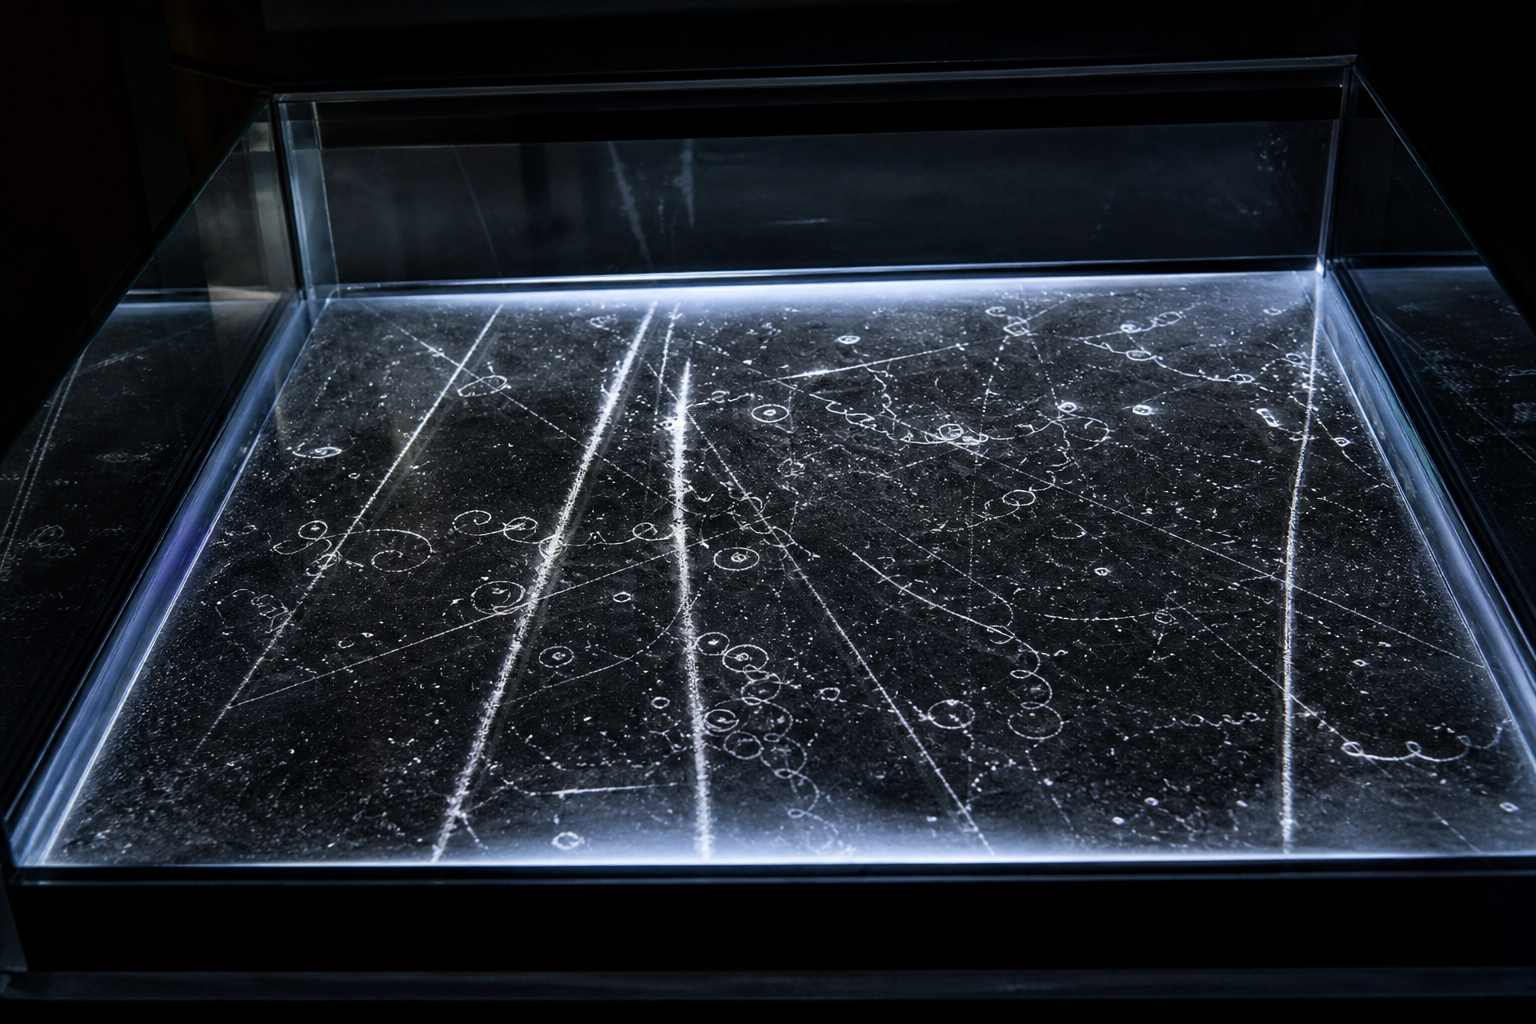
\includegraphics[width=0.58\linewidth]{images/book5/ai/b5-05-cloud-chamber.png}

{\small Des particules chargées traversant une chambre à brouillard. Des traces comme celles-ci --- s'enroulant dans les champs magnétiques, apparaissant par paires --- ont fait de $E = mc^2$ une comptabilité quotidienne~: le positon a été découvert sur une telle photographie.}
\end{omfigure}

\section{Exercices}

\begin{exercise}[$\star$]\label{exo:b3:relativistic-dynamics:1}
Un électron ($mc^2 = \qty{0.511}{MeV}$) va à $0.99c$. Calculer
$\gamma$, sa quantité de mouvement en $\unit{MeV}/c$, son énergie
totale et son énergie cinétique. Mêmes questions pour un proton
($mc^2 = \qty{938}{MeV}$) d'énergie cinétique \qty{1}{GeV}.
\end{exercise}

\begin{exercise}[$\star$]\label{exo:b3:relativistic-dynamics:2}
(a) Combien d'énergie dort dans un gramme de matière~? (b) L'explosion
d'Hiroshima a libéré environ \qty{6e13}{J}~: quelle différence de masse
cela fait-il~? (c) Le Soleil rayonne $L = \qty{3.8e26}{W}$~: quelle
masse perd-il par seconde, et quelle fraction de ses $\qty{2e30}{kg}$
en dix milliards d'années~? (d) La batterie de votre téléphone stocke
\qty{5e4}{J}~: de combien un téléphone chargé est-il plus lourd~?
\end{exercise}

\begin{exercise}[$\star$]\label{exo:b3:relativistic-dynamics:3}
(a) Quelle quantité de mouvement le faisceau d'un pointeur laser de
\qty{5}{mW} emporte-t-il par seconde, et quelle force le pointeur
ressent-il~? (b) Quelle force la lumière solaire (\qty{1.4}{kW/m^2})
exerce-t-elle sur une voile solaire parfaitement réfléchissante de
\qty{100}{m^2}~? (c) Partant du repos, à quelle vitesse va un
voilier de \qty{10}{kg} après un mois~? (d) Pourquoi la queue de
poussière d'une comète pointe-t-elle à l'opposé du Soleil~?
\end{exercise}

\begin{exercise}[$\star$]\label{exo:b3:relativistic-dynamics:4}
Exercice d'unités. (a) Montrer que $\unit{MeV}/c^2$ est une unité de
masse et convertir la masse de l'électron en kilogrammes. (b) Que
vaut \qty{1}{GeV/c} en $\unit{kg.m/s}$~? (c) Un carré de \omterm{def:b3:relativistic-dynamics:four-momentum}{masse
invariante} vaut $s = \qty{16}{GeV^2}$ (en unités $c = 1$)~: quelle
énergie de centre de masse est-ce~? (d) Pourquoi les physiciens des
particules posent-ils $c = 1$, et que doit réinsérer un lecteur pour
obtenir des nombres SI~?
\end{exercise}

\begin{exercise}[$\star\star$]\label{exo:b3:relativistic-dynamics:5}
Les électrons de Bertozzi avaient des énergies cinétiques de $0.5$,
$1$, $4.5$ et \qty{15}{MeV}. (a) Calculer la prédiction de Newton
$v^2 = 2E_k/m$ pour chacune, en unités de $c^2$. (b) Calculer le
$v^2/c^2$ relativiste. (c) Son temps de vol sur \qty{8.4}{m} à
\qty{15}{MeV}~: qu'indiqua le chronomètre, et qu'aurait prédit
Newton~? (d) L'énergie des électrons était aussi mesurée par
calorimétrie --- par leur chaleur à l'impact~: pourquoi cette étape
était-elle le vrai enjeu de l'expérience~?
\end{exercise}

\begin{exercise}[$\star\star$]\label{exo:b3:relativistic-dynamics:6}
Le pion chargé se désintègre au repos~: $\pi^+ \to \mu^+\nu$, $m_\pi c^2 =
\qty{139.6}{MeV}$, $m_\mu c^2 = \qty{105.7}{MeV}$, $m_\nu \approx 0$.
(a) Montrer que $pc = (m_\pi^2 - m_\mu^2)c^4/2m_\pi c^2$ et l'évaluer.
(b) L'énergie cinétique et la vitesse du muon. (c) L'énergie du
neutrino. (d) En vol à $\gamma_\pi = 50$, quelles sont les énergies
maximale et minimale du muon de désintégration au laboratoire
(désintégration vers l'avant et vers l'arrière)~?
\end{exercise}

\begin{exercise}[$\star\star$]\label{exo:b3:relativistic-dynamics:7}
La \omterm{def:b3:relativistic-dynamics:four-momentum}{masse invariante} à l'œuvre. (a) Deux photons de \qty{200}{MeV}
chacun volent à $60^\circ$ l'un de l'autre~: calculer la \omterm{def:b3:relativistic-dynamics:four-momentum}{masse
invariante} de la paire. (b) Un pion neutre ($m_{\pi^0}c^2 = \qty{135}{MeV}$)
se désintègre en deux photons~: quelle est la \omterm{def:b3:relativistic-dynamics:four-momentum}{masse invariante} de la
paire de photons, dans tout référentiel~? (c) Expliquer comment une
expérience «~découvre~» une particule sous forme d'une bosse dans la
distribution de \omterm{def:b3:relativistic-dynamics:four-momentum}{masse invariante} de ses produits de désintégration. (d)
Deux photons de même énergie volent exactement parallèlement~: \omterm{def:b3:relativistic-dynamics:four-momentum}{masse
invariante}~? Que dit cela du référentiel propre d'un faisceau lumineux~?
\end{exercise}

\begin{exercise}[$\star\star$]\label{exo:b3:relativistic-dynamics:8}
Comptabilité du LHC (protons de $E = \qty{6.8}{TeV}$). (a) $\gamma$, et
le déficit de vitesse $c - v$ (utiliser $c - v \approx c/2\gamma^2$).
(b) La fréquence de révolution sur l'anneau de \qty{27}{km} et le
nombre de tours par seconde. (c) L'énergie stockée dans un faisceau de
\num{3e14} protons, en kilogrammes de TNT (\qty{4.2e6}{J/kg}). (d)
L'équivalent en masse de l'énergie cinétique des deux faisceaux, en
microgrammes --- de la matière sur le point d'être faite.
\end{exercise}

\begin{exercise}[$\star\star$]\label{exo:b3:relativistic-dynamics:9}
Photons en collision. (a) Montrer qu'un photon isolé dans le vide ne
peut pas se désintégrer en une paire électron--positon, si énergétique
soit-il (utiliser l'invariant). (b) Contre un second photon d'énergie
$\epsilon$ en collision frontale, montrer que la création de paire
exige $E\epsilon \ge (m_{\text{e}}c^2)^2$. (c) Un photon de
\qty{511}{keV} demande quel partenaire~? Un rayon X de \qty{50}{keV}~?
(d) L'univers est empli de lumière stellaire et du fond diffus
micro-onde~: que prédit (b) pour la portée des rayons $\gamma$ du TeV à
travers l'espace intergalactique~?
\end{exercise}

\begin{exercise}[$\star\star\star$]\label{exo:b3:relativistic-dynamics:10}
Compton, par les quadrivecteurs. Un photon de longueur d'onde $\lambda$
frappe un électron au repos et diffuse sous l'angle $\theta$. (a)
Écrire la conservation du \omterm{def:b3:relativistic-dynamics:four-momentum}{quadrivecteur énergie--impulsion} et isoler
l'invariant de l'électron final. (b) Obtenir
\[
\lambda' - \lambda = \frac{h}{m_{\text{e}}c}\,(1 - \cos\theta) .
\]
(c) Évaluer $h/m_{\text{e}}c$ et le décalage maximal~; pourquoi l'effet
est-il invisible en lumière visible mais décisif pour les rayons X~?
(d) Qu'établit la mesure de Compton en 1923 au sujet de la lumière que
l'effet photoélectrique n'avait pas établi~?
\end{exercise}

\begin{exercise}[$\star\star\star$]\label{exo:b3:relativistic-dynamics:11}
La fin du spectre des rayons cosmiques. L'univers baigne dans des
photons micro-ondes d'énergie typique $\epsilon = \qty{6e-4}{eV}$. Un
proton d'énergie $E$ en frappant un de front peut être excité en
résonance $\Delta$ ($m_\Delta c^2 = \qty{1232}{MeV}$), perdant de
l'énergie à chaque fois. (a) Montrer que la condition de seuil s'écrit approximativement $4E\epsilon =
(m_\Delta^2 - m_{\text{p}}^2)c^4$. (b) Calculer le seuil $E$. (c)
Au-dessus, l'univers est opaque aux protons au-delà de quelque
\qty{100}{Mly}~: que prédit cela pour le spectre observé des rayons
cosmiques (la coupure de Greisen--Zatsepin--Kuzmin)~? (d) Des rayons
cosmiques de $\qty{3e20}{eV}$ ont été enregistrés --- les particules
«~Oh-My-God~»~: qu'exige leur existence de leurs sources~?
\end{exercise}

\begin{exercise}[$\star\star\star$]\label{exo:b3:relativistic-dynamics:12}
La fusée à photons. Une fusée de masse initiale $m_{\text{i}}$ éjecte
son échappement sous forme d'un faisceau lumineux collimaté et atteint
la vitesse $\beta c$. (a) En conservant l'énergie et la quantité de
mouvement entre le départ et l'arrivée, montrer que
\[
\frac{m_{\text{i}}}{m_{\text{f}}} =
\sqrt{\frac{1 + \beta}{1 - \beta}} = \eu^{\varphi} ,
\]
l'exponentielle de la rapidité --- l'équation de Tsiolkovski
relativiste avec le meilleur échappement possible. (b) Rapport de
masses pour atteindre $0.9c$~? Et pour atteindre $0.9c$ puis
\emph{s'arrêter} à destination~? (c) Il faut bien fabriquer ce
faisceau~: avec une annihilation matière--antimatière de rendement
parfait, combien de kilogrammes d'antimatière par kilogramme de charge
utile pour l'aller simple à $0.9c$~? (d) La production mondiale
d'antiprotons se compte en nanogrammes par an~: conclure, en une
phrase, sur les fusées à photons.
\end{exercise}

\begin{omfigure}
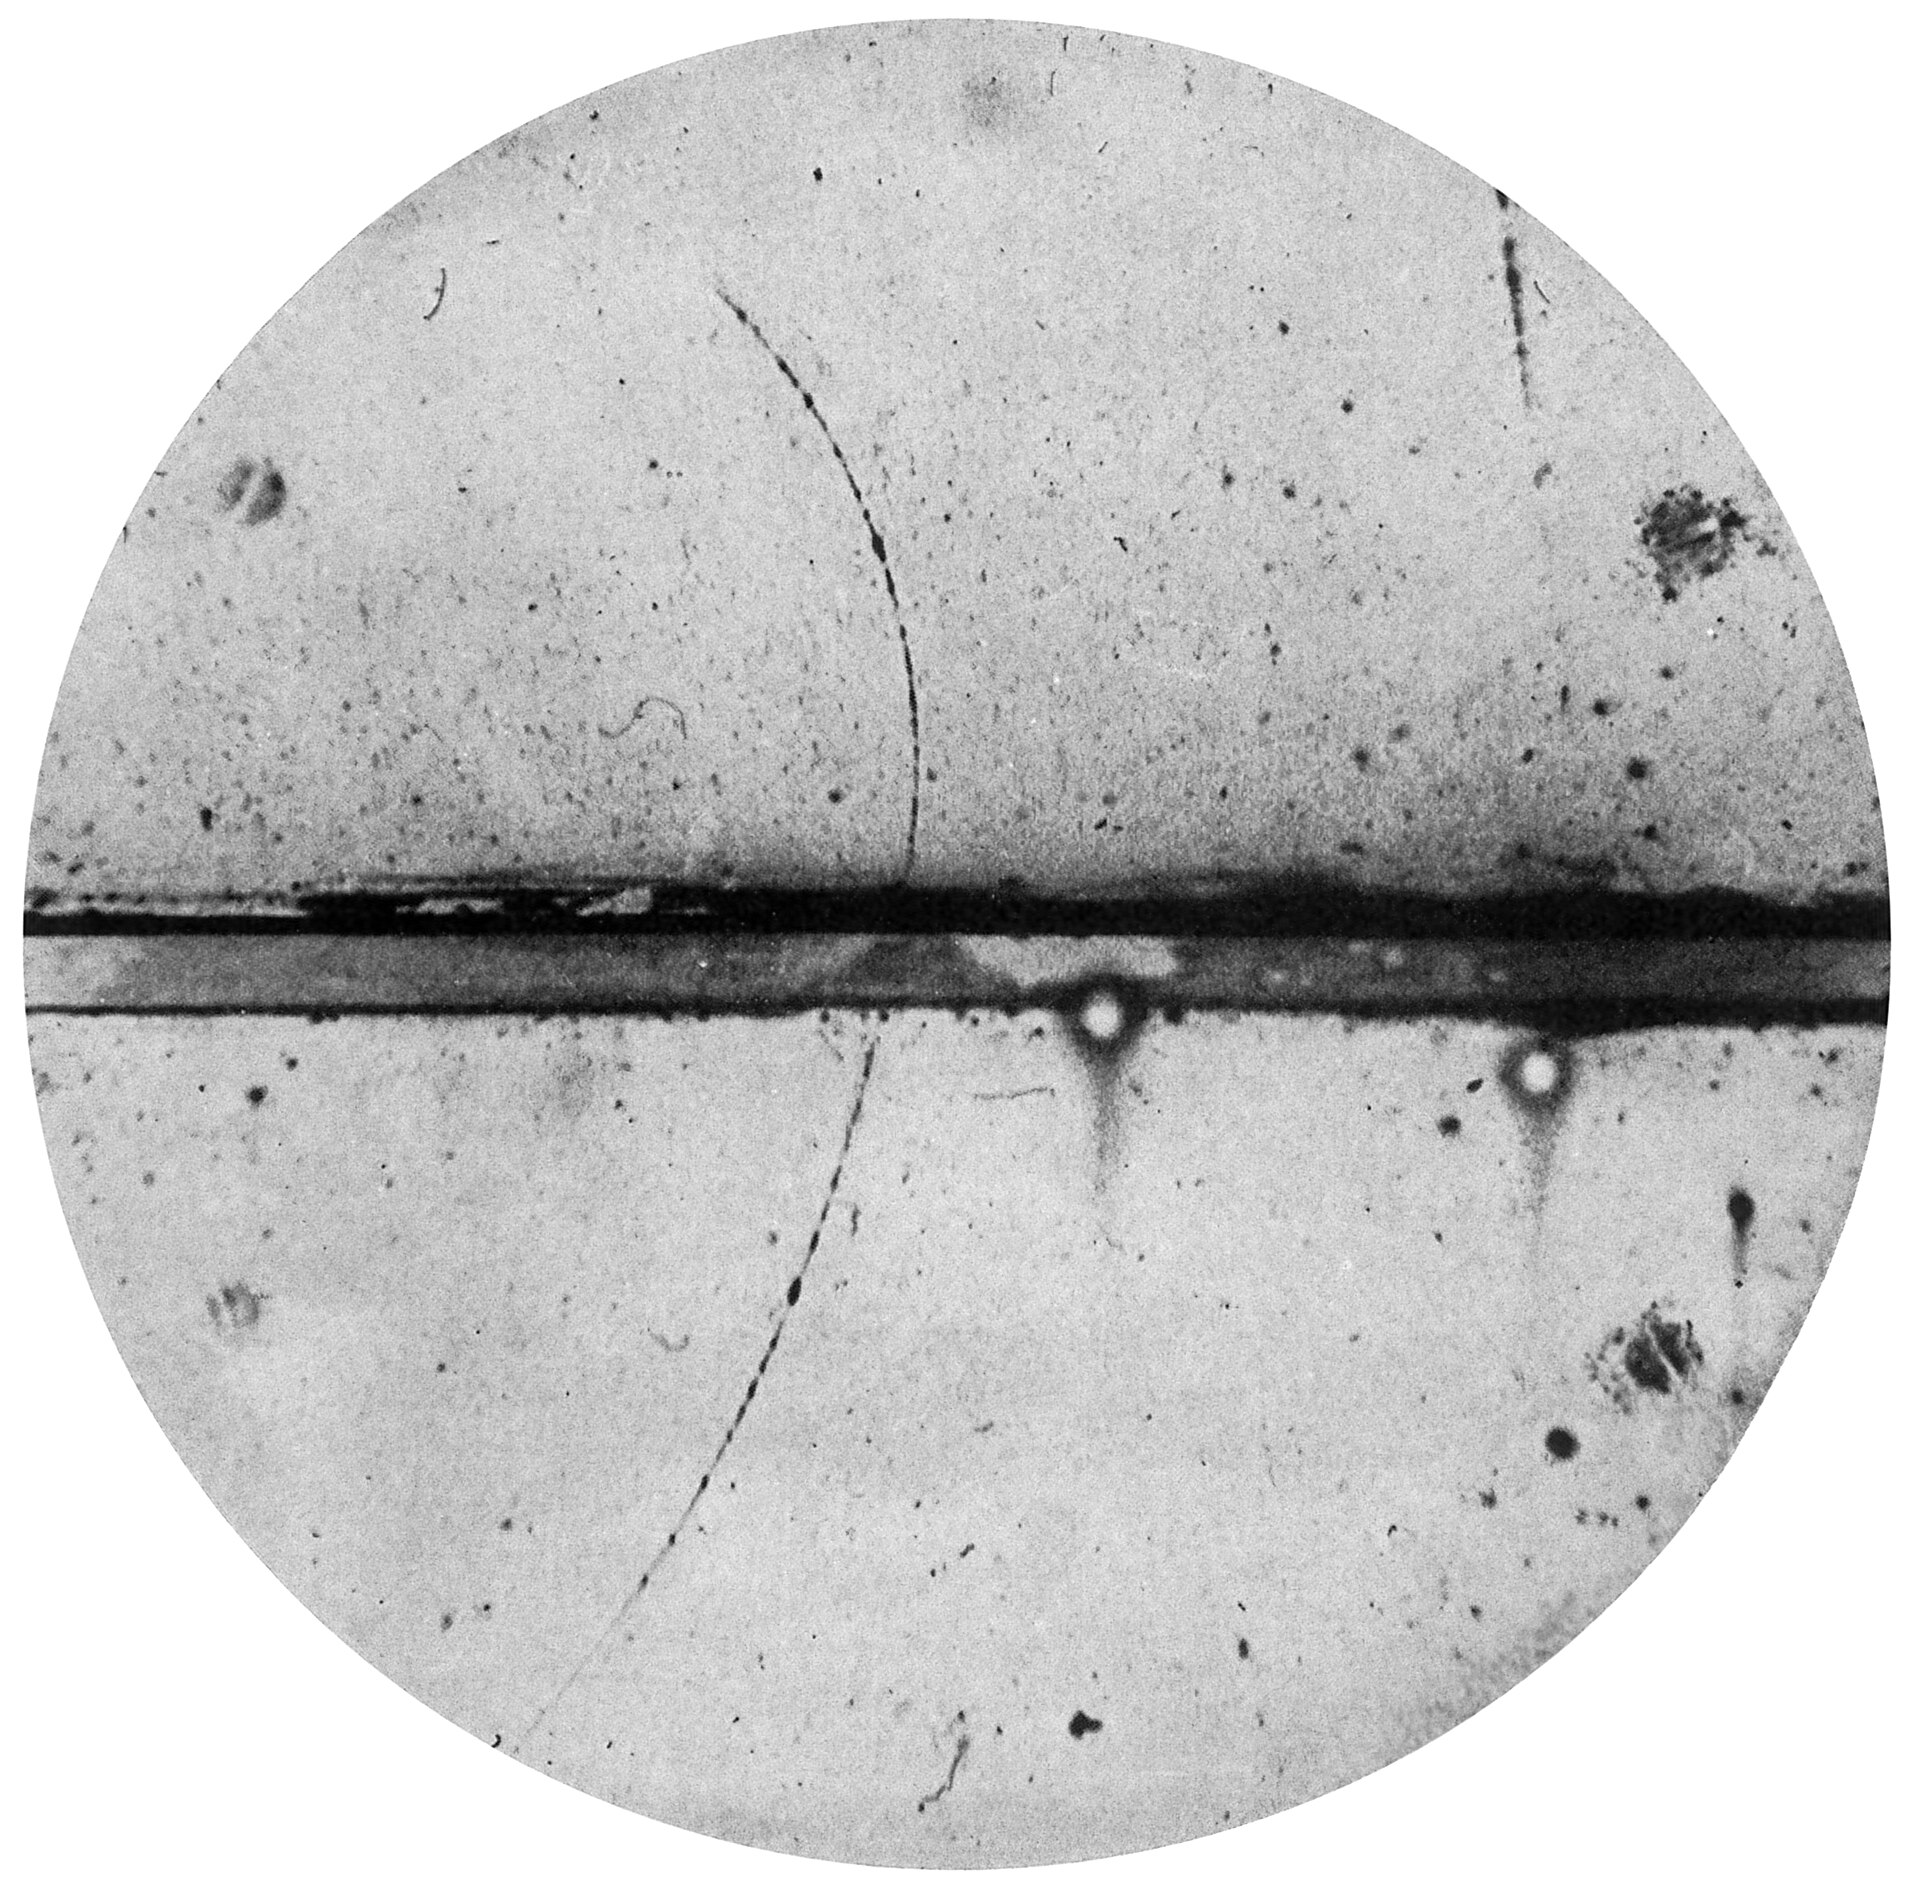
\includegraphics[width=0.5\linewidth]{images/book5/photo-positron-anderson.jpg}

{\small La découverte de l'antimatière (Carl D. Anderson, 1932, domaine public)~: un unique positon montant à travers la plaque de plomb de la chambre à brouillard, courbé du mauvais côté pour un électron et trop serré pour un proton --- le grand livre de $E = mc^2$ pris à tourner à l'envers.}
\end{omfigure}

\section{Problème~: fabriquer de la matière --- l'antiproton et le Bevatron}

\begin{problem}[{Problème du week-end --- comment la conservation de la
quantité de mouvement a fixé le prix de l'antimonde}]\label{pb:b3:relativistic-dynamics:1}
Les équations de Dirac exigeaient, dès 1931, que le proton eût un
jumeau en miroir de charge opposée. En fabriquer un signifiait acheter
son \omterm{def:b3:relativistic-dynamics:momentum-energy}{énergie de masse} avec de l'énergie de faisceau --- et la
conservation de la quantité de mouvement en fixait le prix. Ce problème
en établit le tarif, conçoit la machine qui l'a payé et suit la
découverte de 1955. Données~: $m_{\text{p}}c^2 = \qty{938.3}{MeV}$~; la
charge et le \emph{nombre baryonique} (protons et neutrons $+1$,
antiprotons $-1$) sont conservés dans toute réaction.

\medskip\noindent\textbf{Partie I --- La boîte à outils du quadrivecteur.}
\begin{enumerate}
  \item Pour une particule, montrer que $E^2 - p^2c^2 = m^2c^4$ à
        partir des définitions de $E$ et $\vect p$.
  \item Pour un système, pourquoi $E_{\text{tot}}^2 -
        p_{\text{tot}}^2c^2$ est-il le même dans tous les
        référentiels, et que vaut-il dans le référentiel du centre de
        masse~?
  \item Un faisceau de protons d'énergie $E$ frappe un proton au
        repos~: montrer que
        $M^2c^4 = 2m_{\text{p}}^2c^4 + 2E\,m_{\text{p}}c^2$.
  \item Vérifier les deux limites~: à basse énergie $Mc^2 \to
        2m_{\text{p}}c^2$~; à haute énergie $Mc^2 \approx
        \sqrt{2E\,m_{\text{p}}c^2}$ --- la loi en racine carrée.
  \item Une réaction n'est permise que si $Mc^2$ atteint la somme des
        masses au repos des produits, tous les produits étant au repos
        dans le référentiel du centre de masse au seuil~: justifier
        cette dernière clause.
  \item Pourquoi l'énergie cinétique des produits au laboratoire ne
        peut-elle jamais être récupérée pour créer des particules sur
        une cible fixe~?
\end{enumerate}

\medskip\noindent\textbf{Partie II --- Le prix de l'antiproton.}
\begin{enumerate}[resume]
  \item Dans les collisions $p + p$, la réaction la moins chère
        fabriquant un antiproton $\bar p$ doit aussi fabriquer un
        proton \emph{supplémentaire}~: l'écrire et la justifier par
        la charge et le nombre baryonique.
  \item Montrer que le seuil exige $Mc^2 = 4m_{\text{p}}c^2$.
  \item En déduire l'énergie de faisceau requise $E = 7m_{\text{p}}c^2$
        et l'énergie cinétique $T = 6m_{\text{p}}c^2$~; évaluer $T$.
  \item Au seuil, quelle fraction de l'énergie cinétique du faisceau
        est réellement devenue de la masse au repos nouvelle (dont
        $2m_{\text{p}}c^2$)~? Où est le reste~?
  \item Dans un collisionneur frontal $p$--$p$, quelle énergie
        cinétique \emph{par faisceau} la même réaction demanderait-elle~?
        Comparer les deux conceptions.
  \item En 1954 aucun collisionneur n'existait (les faisceaux étaient
        trop ténus pour se toucher)~: quel fait pratique a imposé le
        choix de la cible fixe, et qu'a-t-il coûté en énergie de
        faisceau~?
\end{enumerate}

\medskip\noindent\textbf{Partie III --- Concevoir le Bevatron.}
La machine construite à Berkeley atteignit $T = \qty{6.2}{GeV}$ ---
confortablement au-dessus du seuil --- avec des champs dipolaires de $B =
\qty{1.56}{T}$.
\begin{enumerate}[resume]
  \item Calculer l'énergie totale et la quantité de mouvement du
        faisceau à son énergie maximale.
  \item Calculer le rayon de courbure $r = p/qB$ et comparer aux
        \qty{15.2}{m} de la machine.
  \item Calculer la vitesse du proton et la fréquence de révolution
        sur l'anneau de longueur $2\pi r$.
  \item À l'injection, les protons arrivent à \qty{10}{MeV}
        d'énergie cinétique~: calculer leur vitesse et expliquer
        pourquoi la fréquence accélératrice devait \emph{balayer}
        pendant chaque cycle (quelles deux grandeurs changent quand
        $E$ croît~?).
  \item Avec environ \qty{1.5}{kV} gagnés par tour, combien de tours
        et combien de temps dure un cycle d'accélération~?
  \item Le nom «~Bevatron~» venait de BeV, milliards d'électronvolts~:
        dites en une ligne quelle physique a fixé le chiffre de
        conception de $6$ et quelques BeV.
\end{enumerate}

\medskip\noindent\textbf{Partie IV --- La découverte, 1955.}
\begin{enumerate}[resume]
  \item Un aimant courbe chaque candidat sur un cercle~: expliquer
        pourquoi cela sélectionne les particules par leur
        \emph{quantité de mouvement} ($r = p/qB$), et non par leur
        énergie ou leur vitesse --- et pourquoi un faisceau ainsi
        sélectionné mélange encore les espèces.
  \item Le faisceau sur une cible de cuivre produisait des torrents de
        pions négatifs ($m_\pi c^2 = \qty{139.6}{MeV}$) parmi lesquels
        se cachaient quelques antiprotons. Le spectromètre sélectionnait
        les négatifs de quantité de mouvement $p = \qty{1.19}{GeV}/c$~:
        calculer la vitesse d'un antiproton et celle d'un pion à cette
        quantité de mouvement.
  \item Sur les \qty{12}{m} de vol, calculer les deux temps de
        parcours~: quelle résolution temporelle la découverte
        exigeait-elle~?
  \item Une seconde signature indépendante utilisait des compteurs
        Tcherenkov, ne se déclenchant qu'au-dessus d'un seuil de
        vitesse~: quelle particule fut-elle réglée pour les
        déclencher, et pourquoi la redondance importe-t-elle à une
        découverte~?
  \item Chamberlain et Segrè comptèrent environ un antiproton pour
        $\num{44000}$ pions~: pourquoi l'argument de seuil
        garantissait-il un taux minuscule même au-dessus du seuil~?
  \item Un antiproton finit par rencontrer un proton et s'annihile~:
        quelle énergie est libérée par événement, et sous quelle forme,
        typiquement~?
  \item Résumer le résultat nommé~: la conservation du \omterm{def:b3:relativistic-dynamics:four-momentum}{quadrivecteur
        énergie--impulsion} a fixé le prix de l'antiproton à $T = 6m_{\text{p}}c^2 =
        \qty{5.6}{GeV}$ sur cible fixe~; un synchrotron de
        \qty{6.2}{GeV} et \qty{15}{m} l'a payé, et l'antimonde est
        devenu un fait de laboratoire --- le prix Nobel de 1959.
\end{enumerate}
\end{problem}
